% Options for packages loaded elsewhere
\PassOptionsToPackage{unicode}{hyperref}
\PassOptionsToPackage{hyphens}{url}
%
\documentclass[
]{article}
\usepackage{amsmath,amssymb}
\usepackage{lmodern}
\usepackage{iftex}
\ifPDFTeX
  \usepackage[T1]{fontenc}
  \usepackage[utf8]{inputenc}
  \usepackage{textcomp} % provide euro and other symbols
\else % if luatex or xetex
  \usepackage{unicode-math}
  \defaultfontfeatures{Scale=MatchLowercase}
  \defaultfontfeatures[\rmfamily]{Ligatures=TeX,Scale=1}
\fi
% Use upquote if available, for straight quotes in verbatim environments
\IfFileExists{upquote.sty}{\usepackage{upquote}}{}
\IfFileExists{microtype.sty}{% use microtype if available
  \usepackage[]{microtype}
  \UseMicrotypeSet[protrusion]{basicmath} % disable protrusion for tt fonts
}{}
\makeatletter
\@ifundefined{KOMAClassName}{% if non-KOMA class
  \IfFileExists{parskip.sty}{%
    \usepackage{parskip}
  }{% else
    \setlength{\parindent}{0pt}
    \setlength{\parskip}{6pt plus 2pt minus 1pt}}
}{% if KOMA class
  \KOMAoptions{parskip=half}}
\makeatother
\usepackage{xcolor}
\IfFileExists{xurl.sty}{\usepackage{xurl}}{} % add URL line breaks if available
\IfFileExists{bookmark.sty}{\usepackage{bookmark}}{\usepackage{hyperref}}
\hypersetup{
  pdftitle={Untitled},
  hidelinks,
  pdfcreator={LaTeX via pandoc}}
\urlstyle{same} % disable monospaced font for URLs
\usepackage[margin=1in]{geometry}
\usepackage{color}
\usepackage{fancyvrb}
\newcommand{\VerbBar}{|}
\newcommand{\VERB}{\Verb[commandchars=\\\{\}]}
\DefineVerbatimEnvironment{Highlighting}{Verbatim}{commandchars=\\\{\}}
% Add ',fontsize=\small' for more characters per line
\usepackage{framed}
\definecolor{shadecolor}{RGB}{248,248,248}
\newenvironment{Shaded}{\begin{snugshade}}{\end{snugshade}}
\newcommand{\AlertTok}[1]{\textcolor[rgb]{0.94,0.16,0.16}{#1}}
\newcommand{\AnnotationTok}[1]{\textcolor[rgb]{0.56,0.35,0.01}{\textbf{\textit{#1}}}}
\newcommand{\AttributeTok}[1]{\textcolor[rgb]{0.77,0.63,0.00}{#1}}
\newcommand{\BaseNTok}[1]{\textcolor[rgb]{0.00,0.00,0.81}{#1}}
\newcommand{\BuiltInTok}[1]{#1}
\newcommand{\CharTok}[1]{\textcolor[rgb]{0.31,0.60,0.02}{#1}}
\newcommand{\CommentTok}[1]{\textcolor[rgb]{0.56,0.35,0.01}{\textit{#1}}}
\newcommand{\CommentVarTok}[1]{\textcolor[rgb]{0.56,0.35,0.01}{\textbf{\textit{#1}}}}
\newcommand{\ConstantTok}[1]{\textcolor[rgb]{0.00,0.00,0.00}{#1}}
\newcommand{\ControlFlowTok}[1]{\textcolor[rgb]{0.13,0.29,0.53}{\textbf{#1}}}
\newcommand{\DataTypeTok}[1]{\textcolor[rgb]{0.13,0.29,0.53}{#1}}
\newcommand{\DecValTok}[1]{\textcolor[rgb]{0.00,0.00,0.81}{#1}}
\newcommand{\DocumentationTok}[1]{\textcolor[rgb]{0.56,0.35,0.01}{\textbf{\textit{#1}}}}
\newcommand{\ErrorTok}[1]{\textcolor[rgb]{0.64,0.00,0.00}{\textbf{#1}}}
\newcommand{\ExtensionTok}[1]{#1}
\newcommand{\FloatTok}[1]{\textcolor[rgb]{0.00,0.00,0.81}{#1}}
\newcommand{\FunctionTok}[1]{\textcolor[rgb]{0.00,0.00,0.00}{#1}}
\newcommand{\ImportTok}[1]{#1}
\newcommand{\InformationTok}[1]{\textcolor[rgb]{0.56,0.35,0.01}{\textbf{\textit{#1}}}}
\newcommand{\KeywordTok}[1]{\textcolor[rgb]{0.13,0.29,0.53}{\textbf{#1}}}
\newcommand{\NormalTok}[1]{#1}
\newcommand{\OperatorTok}[1]{\textcolor[rgb]{0.81,0.36,0.00}{\textbf{#1}}}
\newcommand{\OtherTok}[1]{\textcolor[rgb]{0.56,0.35,0.01}{#1}}
\newcommand{\PreprocessorTok}[1]{\textcolor[rgb]{0.56,0.35,0.01}{\textit{#1}}}
\newcommand{\RegionMarkerTok}[1]{#1}
\newcommand{\SpecialCharTok}[1]{\textcolor[rgb]{0.00,0.00,0.00}{#1}}
\newcommand{\SpecialStringTok}[1]{\textcolor[rgb]{0.31,0.60,0.02}{#1}}
\newcommand{\StringTok}[1]{\textcolor[rgb]{0.31,0.60,0.02}{#1}}
\newcommand{\VariableTok}[1]{\textcolor[rgb]{0.00,0.00,0.00}{#1}}
\newcommand{\VerbatimStringTok}[1]{\textcolor[rgb]{0.31,0.60,0.02}{#1}}
\newcommand{\WarningTok}[1]{\textcolor[rgb]{0.56,0.35,0.01}{\textbf{\textit{#1}}}}
\usepackage{graphicx}
\makeatletter
\def\maxwidth{\ifdim\Gin@nat@width>\linewidth\linewidth\else\Gin@nat@width\fi}
\def\maxheight{\ifdim\Gin@nat@height>\textheight\textheight\else\Gin@nat@height\fi}
\makeatother
% Scale images if necessary, so that they will not overflow the page
% margins by default, and it is still possible to overwrite the defaults
% using explicit options in \includegraphics[width, height, ...]{}
\setkeys{Gin}{width=\maxwidth,height=\maxheight,keepaspectratio}
% Set default figure placement to htbp
\makeatletter
\def\fps@figure{htbp}
\makeatother
\setlength{\emergencystretch}{3em} % prevent overfull lines
\providecommand{\tightlist}{%
  \setlength{\itemsep}{0pt}\setlength{\parskip}{0pt}}
\setcounter{secnumdepth}{-\maxdimen} % remove section numbering
\ifLuaTeX
  \usepackage{selnolig}  % disable illegal ligatures
\fi

\title{Untitled}
\author{}
\date{\vspace{-2.5em}}

\begin{document}
\maketitle

\hypertarget{r-markdown}{%
\subsection{R Markdown}\label{r-markdown}}

This is an R Markdown document. Markdown is a simple formatting syntax
for authoring HTML, PDF, and MS Word documents. For more details on
using R Markdown see \url{http://rmarkdown.rstudio.com}.

When you click the \textbf{Knit} button a document will be generated
that includes both content as well as the output of any embedded R code
chunks within the document. You can embed an R code chunk like this:

\begin{Shaded}
\begin{Highlighting}[]
\FunctionTok{library}\NormalTok{(}\StringTok{"stargazer"}\NormalTok{)}
\end{Highlighting}
\end{Shaded}

\begin{verbatim}
## 
## Please cite as:
\end{verbatim}

\begin{verbatim}
##  Hlavac, Marek (2018). stargazer: Well-Formatted Regression and Summary Statistics Tables.
\end{verbatim}

\begin{verbatim}
##  R package version 5.2.2. https://CRAN.R-project.org/package=stargazer
\end{verbatim}

\begin{Shaded}
\begin{Highlighting}[]
\FunctionTok{library}\NormalTok{(purrr)}
\FunctionTok{library}\NormalTok{(readr)}
\FunctionTok{library}\NormalTok{(estimatr)}
\FunctionTok{library}\NormalTok{(lmtest)}
\end{Highlighting}
\end{Shaded}

\begin{verbatim}
## Loading required package: zoo
\end{verbatim}

\begin{verbatim}
## 
## Attaching package: 'zoo'
\end{verbatim}

\begin{verbatim}
## The following objects are masked from 'package:base':
## 
##     as.Date, as.Date.numeric
\end{verbatim}

\begin{Shaded}
\begin{Highlighting}[]
\FunctionTok{library}\NormalTok{(sandwich)}
\FunctionTok{library}\NormalTok{(haven)}
\FunctionTok{set.seed}\NormalTok{(}\DecValTok{2021}\NormalTok{)}
\end{Highlighting}
\end{Shaded}

\hypertarget{question-1}{%
\section{Question 1:}\label{question-1}}

\begin{enumerate}
\def\labelenumi{\alph{enumi})}
\tightlist
\item
  Assume that \(\gamma = 1\). Generate 5000 observations and then use
  OLS to estimate the parameters in the model and calculate the related
  OLS standard errors, t-values and p-values. Then use OLS to estimate
  the model with White standard errors1 and calculate the related White
  standard errors, t-values and p-values. Compare the results.
\end{enumerate}

\begin{Shaded}
\begin{Highlighting}[]
\NormalTok{n }\OtherTok{=} \DecValTok{5000}
\NormalTok{b0 }\OtherTok{=} \DecValTok{3}
\NormalTok{b1 }\OtherTok{=} \DecValTok{5}
\NormalTok{b2 }\OtherTok{=} \DecValTok{8}
\NormalTok{x1 }\OtherTok{=} \FunctionTok{rnorm}\NormalTok{(n, }\DecValTok{1}\NormalTok{, }\DecValTok{1}\NormalTok{)}
\NormalTok{x2 }\OtherTok{=} \FunctionTok{rnorm}\NormalTok{(n, }\DecValTok{2}\NormalTok{, }\DecValTok{1}\NormalTok{)}
\NormalTok{z }\OtherTok{=} \FunctionTok{rgamma}\NormalTok{(n, }\FloatTok{1.2}\NormalTok{, }\FloatTok{1.1}\NormalTok{)}
\NormalTok{sigma }\OtherTok{=} \DecValTok{1}
\NormalTok{gamma }\OtherTok{=} \DecValTok{1}
\end{Highlighting}
\end{Shaded}

\begin{Shaded}
\begin{Highlighting}[]
\NormalTok{sigmaV }\OtherTok{=}\NormalTok{ sigma}\SpecialCharTok{*}\FunctionTok{exp}\NormalTok{(gamma}\SpecialCharTok{*}\NormalTok{z)}
\NormalTok{epsilon }\OtherTok{=} \FunctionTok{rnorm}\NormalTok{(n, }\DecValTok{0}\NormalTok{, }\FunctionTok{sqrt}\NormalTok{(sigmaV))}
\FunctionTok{plot}\NormalTok{(epsilon, }\AttributeTok{type =} \StringTok{"l"}\NormalTok{)}
\end{Highlighting}
\end{Shaded}

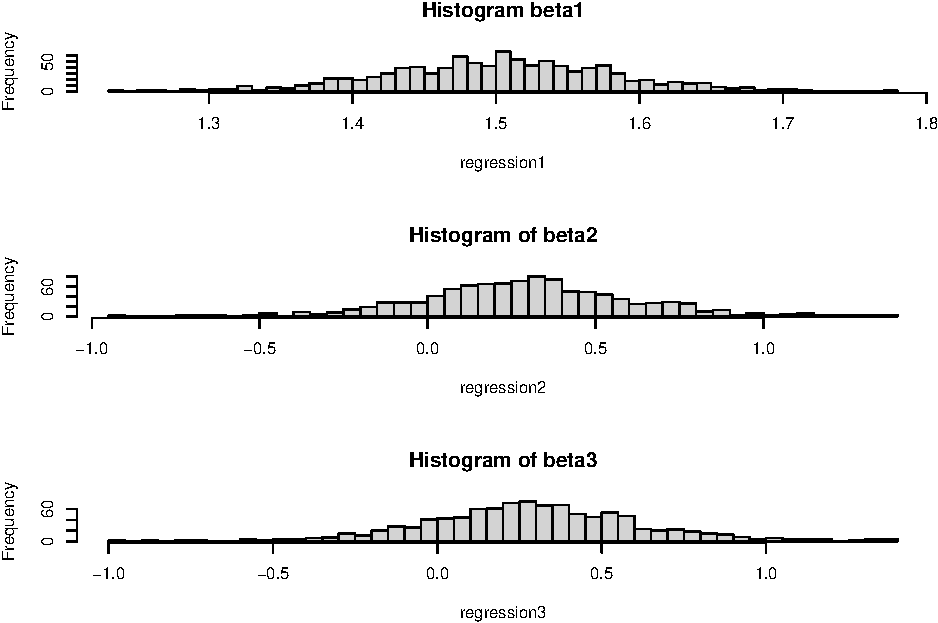
\includegraphics{Aissignment2_files/figure-latex/unnamed-chunk-3-1.pdf}

\begin{Shaded}
\begin{Highlighting}[]
\NormalTok{y }\OtherTok{=}\NormalTok{ b0 }\SpecialCharTok{+}\NormalTok{ b1}\SpecialCharTok{*}\NormalTok{x1 }\SpecialCharTok{+}\NormalTok{ b2}\SpecialCharTok{*}\NormalTok{x2 }\SpecialCharTok{+}\NormalTok{ epsilon}
\NormalTok{data }\OtherTok{=} \FunctionTok{data.frame}\NormalTok{(}\FunctionTok{cbind}\NormalTok{(y, x1, x2))}
\NormalTok{model }\OtherTok{\textless{}{-}} \FunctionTok{lm}\NormalTok{(y }\SpecialCharTok{\textasciitilde{}}\NormalTok{ x1 }\SpecialCharTok{+}\NormalTok{ x2, }\AttributeTok{data=}\NormalTok{data)}
\FunctionTok{summary}\NormalTok{(model)}
\end{Highlighting}
\end{Shaded}

\begin{verbatim}
## 
## Call:
## lm(formula = y ~ x1 + x2, data = data)
## 
## Residuals:
##      Min       1Q   Median       3Q      Max 
## -216.090   -1.007    0.104    1.186   74.573 
## 
## Coefficients:
##             Estimate Std. Error t value Pr(>|t|)    
## (Intercept)  2.83388    0.16279   17.41   <2e-16 ***
## x1           5.00369    0.06495   77.03   <2e-16 ***
## x2           8.03097    0.06627  121.18   <2e-16 ***
## ---
## Signif. codes:  0 '***' 0.001 '**' 0.01 '*' 0.05 '.' 0.1 ' ' 1
## 
## Residual standard error: 4.674 on 4997 degrees of freedom
## Multiple R-squared:  0.805,  Adjusted R-squared:  0.8049 
## F-statistic: 1.032e+04 on 2 and 4997 DF,  p-value: < 2.2e-16
\end{verbatim}

\begin{Shaded}
\begin{Highlighting}[]
\FunctionTok{coeftest}\NormalTok{(model, }\AttributeTok{vcov.=} \FunctionTok{vcovHC}\NormalTok{(model, }\AttributeTok{type=}\StringTok{"HC0"}\NormalTok{))}
\end{Highlighting}
\end{Shaded}

\begin{verbatim}
## 
## t test of coefficients:
## 
##             Estimate Std. Error t value  Pr(>|t|)    
## (Intercept) 2.833880   0.137610  20.593 < 2.2e-16 ***
## x1          5.003686   0.044425 112.631 < 2.2e-16 ***
## x2          8.030965   0.046046 174.412 < 2.2e-16 ***
## ---
## Signif. codes:  0 '***' 0.001 '**' 0.01 '*' 0.05 '.' 0.1 ' ' 1
\end{verbatim}

We used the coeftest function from the lmtest library in combination
with the funtion vcovHC from the sandwhich package to calculate a model
with the White standard errors. The coeftest function calculates the t
test using a heteroskedasticity robust variance-covariance matrix
produced by the vcov function. With ``HCO'' we indicate that we want to
obtain a White standard error (Source:
\url{https://www.r-econometrics.com/methods/hcrobusterrors/}).
\textbackslash{}

Corresponding to the theory, the estimates are unbiased despite
heteroscedasticity. Hence, it is no surprise that the estimates are the
same for both regressions. However, heteroscedasticity causes
inefficiency of the variance which is why the standard error is higher
in the basic OLS regression than in the OLS model with White standard
errors.

\begin{enumerate}
\def\labelenumi{\alph{enumi})}
\setcounter{enumi}{1}
\tightlist
\item
  What are the procedures to perform the Breusch-Pagan test for
  heteroskedasticity? Perform a Breusch-Pagan test for
  heteroskedasticity. Provide the value of the test statistic and
  explain if the null hypothesis is rejected.
\end{enumerate}

In a Breusch-Pagan test the squared OLS residuals are regressed on
variables that may relate to the variance. It is assumed that
heteroscedasticity is driven by \(z_i\). Hence, the null hypothesis is
that \(\gamma_2,...,\gamma_n\) are zero. \textbackslash{}

To perform the test, we have to estimate \(y\) with OLS and compute the
residuals in the first step. Thereafter, we perform an auxiliary
regression of the form
\(e_i^2 = \gamma_1 + \gamma_2 z_{2i} + ... + \gamma_p z{pi} + \eta_i\).
Takiung \(R^2\) of our auxiliary regression, we can calculate
\(LM = n R^2\) for our test statistic.\textbackslash{}

\begin{Shaded}
\begin{Highlighting}[]
\NormalTok{usq }\OtherTok{\textless{}{-}} \FunctionTok{resid}\NormalTok{(model)}\SpecialCharTok{\^{}}\DecValTok{2}
\CommentTok{\# auxiliary regression: dependent variable squared residuals of first regression, explanatory variables are job categories}
\NormalTok{res }\OtherTok{\textless{}{-}} \FunctionTok{lm}\NormalTok{(usq }\SpecialCharTok{\textasciitilde{}}\NormalTok{ z, data)}
\FunctionTok{summary}\NormalTok{(res)}
\end{Highlighting}
\end{Shaded}

\begin{verbatim}
## 
## Call:
## lm(formula = usq ~ z, data = data)
## 
## Residuals:
##    Min     1Q Median     3Q    Max 
##   -704    -68     19     76  45517 
## 
## Coefficients:
##             Estimate Std. Error t value Pr(>|t|)    
## (Intercept) -125.732     14.315  -8.783   <2e-16 ***
## z            135.381      9.714  13.937   <2e-16 ***
## ---
## Signif. codes:  0 '***' 0.001 '**' 0.01 '*' 0.05 '.' 0.1 ' ' 1
## 
## Residual standard error: 681.2 on 4998 degrees of freedom
## Multiple R-squared:  0.03741,    Adjusted R-squared:  0.03722 
## F-statistic: 194.2 on 1 and 4998 DF,  p-value: < 2.2e-16
\end{verbatim}

\begin{Shaded}
\begin{Highlighting}[]
\NormalTok{nres }\OtherTok{\textless{}{-}} \FunctionTok{nobs}\NormalTok{(res)}
\NormalTok{Rsq}\OtherTok{\textless{}{-}}\FunctionTok{summary}\NormalTok{(res)}\SpecialCharTok{$}\NormalTok{r.squared}

\CommentTok{\# test statistic}
\NormalTok{BP }\OtherTok{\textless{}{-}}\NormalTok{ nres}\SpecialCharTok{*}\NormalTok{Rsq}
\NormalTok{BP}
\end{Highlighting}
\end{Shaded}

\begin{verbatim}
## [1] 187.0461
\end{verbatim}

\begin{Shaded}
\begin{Highlighting}[]
\DecValTok{1}\SpecialCharTok{{-}}\FunctionTok{pchisq}\NormalTok{(BP,}\DecValTok{2}\NormalTok{) }
\end{Highlighting}
\end{Shaded}

\begin{verbatim}
## [1] 0
\end{verbatim}

\begin{Shaded}
\begin{Highlighting}[]
\CommentTok{\# reject H0}
\end{Highlighting}
\end{Shaded}

If \(z_i\) would not drive the heteroscedasticity, the model would not
have any explanatory power. Hence, \(R^2\) would be close to zero as
well as LM (or BR as denoted in the code). However, as the result of the
test statistic shows, BR is not close to zero which gives us evidence
that \(z_i\) indeed drives the heteroscedasticity. Therefore, we reject
the null hypothesis. \textbackslash{}

\begin{enumerate}
\def\labelenumi{\alph{enumi})}
\setcounter{enumi}{2}
\tightlist
\item
  Assume that \(\gamma = 0\). Estimate \(\beta_0, \beta_1\) and
  \(\beta_2\) separately using\textbackslash{}
\end{enumerate}

\begin{enumerate}
\def\labelenumi{\arabic{enumi}.}
\tightlist
\item
  OLS\textbackslash{}
\item
  WLS with known \(\gamma = 0\)\textbackslash{}
\item
  FWLS with estimated γ (i.e.~γ is unknown)\textbackslash{}
\end{enumerate}

Explain the weights you use for WLS and FWLS. Provide the coefficients
and standard errors of the three estimators for three methods and
compare the results. Are the estimators close to the their true
values?\textbackslash{}

\begin{Shaded}
\begin{Highlighting}[]
\NormalTok{gammaC }\OtherTok{=} \DecValTok{0}
\NormalTok{sigmaC }\OtherTok{=}\NormalTok{ sigma}\SpecialCharTok{*}\FunctionTok{exp}\NormalTok{(gammaC}\SpecialCharTok{*}\NormalTok{z)}
\NormalTok{epsilonC }\OtherTok{=} \FunctionTok{rnorm}\NormalTok{(n, }\DecValTok{0}\NormalTok{, }\FunctionTok{sqrt}\NormalTok{(sigmaC))}
\FunctionTok{plot}\NormalTok{(epsilonC, }\AttributeTok{type =} \StringTok{"l"}\NormalTok{)}
\end{Highlighting}
\end{Shaded}

\includegraphics{Aissignment2_files/figure-latex/unnamed-chunk-7-1.pdf}

\begin{Shaded}
\begin{Highlighting}[]
\NormalTok{yC }\OtherTok{=}\NormalTok{ b0 }\SpecialCharTok{+}\NormalTok{ b1}\SpecialCharTok{*}\NormalTok{x1 }\SpecialCharTok{+}\NormalTok{ b2}\SpecialCharTok{*}\NormalTok{x2 }\SpecialCharTok{+}\NormalTok{ epsilonC}
\NormalTok{dataC }\OtherTok{=} \FunctionTok{data.frame}\NormalTok{(}\FunctionTok{cbind}\NormalTok{(yC, x1, x2))}
\NormalTok{modelC }\OtherTok{\textless{}{-}} \FunctionTok{lm}\NormalTok{(yC }\SpecialCharTok{\textasciitilde{}}\NormalTok{ x1 }\SpecialCharTok{+}\NormalTok{ x2, }\AttributeTok{data =}\NormalTok{dataC)}
\FunctionTok{summary}\NormalTok{(modelC)}
\end{Highlighting}
\end{Shaded}

\begin{verbatim}
## 
## Call:
## lm(formula = yC ~ x1 + x2, data = dataC)
## 
## Residuals:
##     Min      1Q  Median      3Q     Max 
## -3.2104 -0.6910 -0.0033  0.6863  3.6539 
## 
## Coefficients:
##             Estimate Std. Error t value Pr(>|t|)    
## (Intercept)  2.93799    0.03510   83.71   <2e-16 ***
## x1           5.00834    0.01400  357.64   <2e-16 ***
## x2           8.01890    0.01429  561.22   <2e-16 ***
## ---
## Signif. codes:  0 '***' 0.001 '**' 0.01 '*' 0.05 '.' 0.1 ' ' 1
## 
## Residual standard error: 1.008 on 4997 degrees of freedom
## Multiple R-squared:  0.9889, Adjusted R-squared:  0.9888 
## F-statistic: 2.216e+05 on 2 and 4997 DF,  p-value: < 2.2e-16
\end{verbatim}

For the weighthed least square model, we use \(exp(\gamma z_i)\) as our
weight, as this is the component that drives the heteroskedasticity in
our errors: \(w_i = \frac{1}{e^{\gamma z_i}}\). As \(\gamma = 0\), the
regression should result in the same estimators and same variances as in
the basic OLS regression.

\begin{Shaded}
\begin{Highlighting}[]
\CommentTok{\# {-}{-}{-}{-}{-} WLS}
\NormalTok{w }\OtherTok{\textless{}{-}} \DecValTok{1}\SpecialCharTok{/}\FunctionTok{exp}\NormalTok{(gammaC}\SpecialCharTok{*}\NormalTok{z) }\CommentTok{\# specify weight}
\NormalTok{modelWLS }\OtherTok{\textless{}{-}} \FunctionTok{lm}\NormalTok{(yC }\SpecialCharTok{\textasciitilde{}}\NormalTok{ x1 }\SpecialCharTok{+}\NormalTok{ x2, }\AttributeTok{data =}\NormalTok{dataC, }\AttributeTok{weights=}\NormalTok{w)}

\FunctionTok{summary}\NormalTok{(modelWLS)}\SpecialCharTok{$}\NormalTok{coeff}
\end{Highlighting}
\end{Shaded}

\begin{verbatim}
##             Estimate Std. Error   t value Pr(>|t|)
## (Intercept) 2.937985 0.03509769  83.70881        0
## x1          5.008338 0.01400366 357.64500        0
## x2          8.018896 0.01428827 561.22231        0
\end{verbatim}

For the feasible weighthed least square model, we first use the
residuals of the basic OLS regression to estimate \(\gamma\). Then we
use this estimator to calculate \(exp(\gamma z_i)\) which is then used
as our weight as this is the component which drives the
heteroskedasticity in our errors.

\begin{Shaded}
\begin{Highlighting}[]
\CommentTok{\# {-}{-}{-} FWLS}
\NormalTok{eps }\OtherTok{\textless{}{-}}\NormalTok{ modelC}\SpecialCharTok{$}\NormalTok{residuals}
\NormalTok{modelEps }\OtherTok{\textless{}{-}} \FunctionTok{lm}\NormalTok{(eps }\SpecialCharTok{\textasciitilde{}}\NormalTok{ z)}
\NormalTok{gammaFWLS }\OtherTok{\textless{}{-}}\NormalTok{ modelEps}\SpecialCharTok{$}\NormalTok{coefficient[}\DecValTok{2}\NormalTok{]}
\NormalTok{w }\OtherTok{\textless{}{-}} \DecValTok{1}\SpecialCharTok{/}\FunctionTok{exp}\NormalTok{(gammaFWLS}\SpecialCharTok{*}\NormalTok{z) }\CommentTok{\# specify weight}
\NormalTok{modelFWLS }\OtherTok{\textless{}{-}} \FunctionTok{lm}\NormalTok{(yC }\SpecialCharTok{\textasciitilde{}}\NormalTok{ x1 }\SpecialCharTok{+}\NormalTok{ x2, }\AttributeTok{data =}\NormalTok{dataC, }\AttributeTok{weights=}\NormalTok{w)}

\FunctionTok{summary}\NormalTok{(modelFWLS)}\SpecialCharTok{$}\NormalTok{coeff}
\end{Highlighting}
\end{Shaded}

\begin{verbatim}
##             Estimate Std. Error   t value Pr(>|t|)
## (Intercept) 2.937786 0.03511869  83.65304        0
## x1          5.008082 0.01400596 357.56783        0
## x2          8.018912 0.01429610 560.91621        0
\end{verbatim}

The estimators and variances are approximately equal in all estimated
models (there are minor differences from the fourth digit on). Only the
variance in the feasible weighted least square model is slightly higher.
However, the difference is minimal. For \(x_1, x_2\) the estimators are
very close to their true value. The intercept also close although there
is a higher difference then for the other estimators.\textbackslash{}

\begin{enumerate}
\def\labelenumi{\alph{enumi})}
\setcounter{enumi}{3}
\tightlist
\item
  Now assume that \(\gamma = 1\). Repeat sub-question(c). Provide the
  coefficients and standard errors of the three estimators for three
  methods and compare the results. Are the estimators close to the true
  ones
\end{enumerate}

\begin{Shaded}
\begin{Highlighting}[]
\NormalTok{gammaD }\OtherTok{=} \DecValTok{1}
\NormalTok{sigmaD }\OtherTok{=}\NormalTok{ sigma}\SpecialCharTok{*}\FunctionTok{exp}\NormalTok{(gammaD}\SpecialCharTok{*}\NormalTok{z)}
\NormalTok{epsilonD }\OtherTok{=} \FunctionTok{rnorm}\NormalTok{(n, }\DecValTok{0}\NormalTok{, }\FunctionTok{sqrt}\NormalTok{(sigmaD))}
\FunctionTok{plot}\NormalTok{(epsilonD, }\AttributeTok{type =} \StringTok{"l"}\NormalTok{)}
\end{Highlighting}
\end{Shaded}

\includegraphics{Aissignment2_files/figure-latex/unnamed-chunk-11-1.pdf}

\begin{Shaded}
\begin{Highlighting}[]
\NormalTok{yD }\OtherTok{=}\NormalTok{ b0 }\SpecialCharTok{+}\NormalTok{ b1}\SpecialCharTok{*}\NormalTok{x1 }\SpecialCharTok{+}\NormalTok{ b2}\SpecialCharTok{*}\NormalTok{x2 }\SpecialCharTok{+}\NormalTok{ epsilonD}
\NormalTok{dataD }\OtherTok{=} \FunctionTok{data.frame}\NormalTok{(}\FunctionTok{cbind}\NormalTok{(yD, x1, x2))}
\NormalTok{modelD }\OtherTok{\textless{}{-}} \FunctionTok{lm}\NormalTok{(yD }\SpecialCharTok{\textasciitilde{}}\NormalTok{ x1 }\SpecialCharTok{+}\NormalTok{ x2, }\AttributeTok{data =}\NormalTok{dataD)}
\FunctionTok{summary}\NormalTok{(modelD)}
\end{Highlighting}
\end{Shaded}

\begin{verbatim}
## 
## Call:
## lm(formula = yD ~ x1 + x2, data = dataD)
## 
## Residuals:
##     Min      1Q  Median      3Q     Max 
## -62.696  -1.117  -0.031   1.051  63.751 
## 
## Coefficients:
##             Estimate Std. Error t value Pr(>|t|)    
## (Intercept)  3.04556    0.10044   30.32   <2e-16 ***
## x1           4.98751    0.04008  124.45   <2e-16 ***
## x2           7.99606    0.04089  195.55   <2e-16 ***
## ---
## Signif. codes:  0 '***' 0.001 '**' 0.01 '*' 0.05 '.' 0.1 ' ' 1
## 
## Residual standard error: 2.884 on 4997 degrees of freedom
## Multiple R-squared:  0.915,  Adjusted R-squared:  0.9149 
## F-statistic: 2.688e+04 on 2 and 4997 DF,  p-value: < 2.2e-16
\end{verbatim}

\begin{Shaded}
\begin{Highlighting}[]
\CommentTok{\# {-}{-}{-}{-}{-} WLS}
\NormalTok{w }\OtherTok{\textless{}{-}} \DecValTok{1}\SpecialCharTok{/}\FunctionTok{exp}\NormalTok{(gammaD}\SpecialCharTok{*}\NormalTok{z) }\CommentTok{\# specify weight}
\NormalTok{modelWLSd }\OtherTok{\textless{}{-}} \FunctionTok{lm}\NormalTok{(yD }\SpecialCharTok{\textasciitilde{}}\NormalTok{ x1 }\SpecialCharTok{+}\NormalTok{ x2, }\AttributeTok{data =}\NormalTok{dataD, }\AttributeTok{weights=}\NormalTok{w)}

\FunctionTok{summary}\NormalTok{(modelWLSd)}\SpecialCharTok{$}\NormalTok{coeff}
\end{Highlighting}
\end{Shaded}

\begin{verbatim}
##             Estimate Std. Error   t value Pr(>|t|)
## (Intercept) 3.007112 0.05114675  58.79381        0
## x1          5.019518 0.02065300 243.04060        0
## x2          7.987665 0.02086295 382.86359        0
\end{verbatim}

This model is not right yet!!!!

\begin{Shaded}
\begin{Highlighting}[]
\CommentTok{\# {-}{-}{-} FWLS}
\NormalTok{epsD }\OtherTok{\textless{}{-}}\NormalTok{ modelD}\SpecialCharTok{$}\NormalTok{residuals}
\NormalTok{modelEpsD }\OtherTok{\textless{}{-}} \FunctionTok{lm}\NormalTok{(epsD }\SpecialCharTok{\textasciitilde{}}\NormalTok{ z)}
\NormalTok{gammaFWLSD }\OtherTok{\textless{}{-}}\NormalTok{ modelEpsD}\SpecialCharTok{$}\NormalTok{coefficient[}\DecValTok{2}\NormalTok{]}
\NormalTok{w }\OtherTok{\textless{}{-}} \DecValTok{1}\SpecialCharTok{/}\FunctionTok{exp}\NormalTok{(gammaFWLSD}\SpecialCharTok{*}\NormalTok{z) }\CommentTok{\# specify weight}
\NormalTok{modelFWLSD }\OtherTok{\textless{}{-}} \FunctionTok{lm}\NormalTok{(yD }\SpecialCharTok{\textasciitilde{}}\NormalTok{ x1 }\SpecialCharTok{+}\NormalTok{ x2, }\AttributeTok{data =}\NormalTok{dataD, }\AttributeTok{weights=}\NormalTok{w)}

\FunctionTok{summary}\NormalTok{(modelFWLSD)}\SpecialCharTok{$}\NormalTok{coeff}
\end{Highlighting}
\end{Shaded}

\begin{verbatim}
##             Estimate Std. Error   t value      Pr(>|t|)
## (Intercept) 3.041220 0.09000512  33.78941 1.347516e-225
## x1          4.992763 0.03596599 138.81900  0.000000e+00
## x2          7.992923 0.03664916 218.09295  0.000000e+00
\end{verbatim}

The estimators of all three models are very close to the true values.
However, the variance is higher in the basic OLS model than in the WLS
and FWLS models which is not surprising given the heteroskedasticity of
the errors.

\begin{enumerate}
\def\labelenumi{\alph{enumi})}
\setcounter{enumi}{4}
\tightlist
\item
  Now assume that \(\gamma = −1\). Repeat sub-question(c). Provide the
  coefficients and standard errors of the three estimators for three
  methods and compare the results. Are the estimators close to the true
  ones?
\end{enumerate}

\begin{Shaded}
\begin{Highlighting}[]
\NormalTok{gammaE }\OtherTok{=} \DecValTok{0}
\NormalTok{sigmaE }\OtherTok{=}\NormalTok{ sigma}\SpecialCharTok{*}\FunctionTok{exp}\NormalTok{(gammaE}\SpecialCharTok{*}\NormalTok{z)}
\NormalTok{epsilonE }\OtherTok{=} \FunctionTok{rnorm}\NormalTok{(n, }\DecValTok{0}\NormalTok{, }\FunctionTok{sqrt}\NormalTok{(sigmaE))}
\FunctionTok{plot}\NormalTok{(epsilonE, }\AttributeTok{type =} \StringTok{"l"}\NormalTok{)}
\end{Highlighting}
\end{Shaded}

\includegraphics{Aissignment2_files/figure-latex/unnamed-chunk-15-1.pdf}

\begin{Shaded}
\begin{Highlighting}[]
\NormalTok{yE }\OtherTok{=}\NormalTok{ b0 }\SpecialCharTok{+}\NormalTok{ b1}\SpecialCharTok{*}\NormalTok{x1 }\SpecialCharTok{+}\NormalTok{ b2}\SpecialCharTok{*}\NormalTok{x2 }\SpecialCharTok{+}\NormalTok{ epsilonE}
\NormalTok{dataE }\OtherTok{=} \FunctionTok{data.frame}\NormalTok{(}\FunctionTok{cbind}\NormalTok{(yE, x1, x2))}
\NormalTok{modelE }\OtherTok{\textless{}{-}} \FunctionTok{lm}\NormalTok{(yE }\SpecialCharTok{\textasciitilde{}}\NormalTok{ x1 }\SpecialCharTok{+}\NormalTok{ x2, }\AttributeTok{data =}\NormalTok{dataE)}
\FunctionTok{summary}\NormalTok{(modelE)}
\end{Highlighting}
\end{Shaded}

\begin{verbatim}
## 
## Call:
## lm(formula = yE ~ x1 + x2, data = dataE)
## 
## Residuals:
##     Min      1Q  Median      3Q     Max 
## -3.6915 -0.6789 -0.0164  0.6799  3.6456 
## 
## Coefficients:
##             Estimate Std. Error t value Pr(>|t|)    
## (Intercept)  2.98275    0.03460   86.21   <2e-16 ***
## x1           4.97856    0.01380  360.66   <2e-16 ***
## x2           8.02233    0.01408  569.58   <2e-16 ***
## ---
## Signif. codes:  0 '***' 0.001 '**' 0.01 '*' 0.05 '.' 0.1 ' ' 1
## 
## Residual standard error: 0.9934 on 4997 degrees of freedom
## Multiple R-squared:  0.9891, Adjusted R-squared:  0.9891 
## F-statistic: 2.274e+05 on 2 and 4997 DF,  p-value: < 2.2e-16
\end{verbatim}

\begin{Shaded}
\begin{Highlighting}[]
\CommentTok{\# {-}{-}{-}{-}{-} WLS}
\NormalTok{w }\OtherTok{\textless{}{-}} \DecValTok{1}\SpecialCharTok{/}\FunctionTok{exp}\NormalTok{(gammaE}\SpecialCharTok{*}\NormalTok{z) }\CommentTok{\# specify weight}
\NormalTok{modelWLSe }\OtherTok{\textless{}{-}} \FunctionTok{lm}\NormalTok{(yE }\SpecialCharTok{\textasciitilde{}}\NormalTok{ x1 }\SpecialCharTok{+}\NormalTok{ x2, }\AttributeTok{data =}\NormalTok{dataE, }\AttributeTok{weights=}\NormalTok{w)}

\FunctionTok{summary}\NormalTok{(modelWLSe)}\SpecialCharTok{$}\NormalTok{coeff}
\end{Highlighting}
\end{Shaded}

\begin{verbatim}
##             Estimate Std. Error   t value Pr(>|t|)
## (Intercept) 2.982747 0.03459735  86.21316        0
## x1          4.978565 0.01380403 360.66033        0
## x2          8.022327 0.01408458 569.58213        0
\end{verbatim}

\begin{Shaded}
\begin{Highlighting}[]
\CommentTok{\# {-}{-}{-} FWLS}
\NormalTok{epsE }\OtherTok{\textless{}{-}}\NormalTok{ modelE}\SpecialCharTok{$}\NormalTok{residuals}
\NormalTok{modelEpsE }\OtherTok{\textless{}{-}} \FunctionTok{lm}\NormalTok{(epsE }\SpecialCharTok{\textasciitilde{}}\NormalTok{ z)}
\NormalTok{gammaFWLSE }\OtherTok{\textless{}{-}}\NormalTok{ modelEpsE}\SpecialCharTok{$}\NormalTok{coefficient[}\DecValTok{2}\NormalTok{]}
\NormalTok{w }\OtherTok{\textless{}{-}} \DecValTok{1}\SpecialCharTok{/}\FunctionTok{exp}\NormalTok{(gammaFWLSE}\SpecialCharTok{*}\NormalTok{z) }\CommentTok{\# specify weight}
\NormalTok{modelFWLSE }\OtherTok{\textless{}{-}} \FunctionTok{lm}\NormalTok{(yE }\SpecialCharTok{\textasciitilde{}}\NormalTok{ x1 }\SpecialCharTok{+}\NormalTok{ x2, }\AttributeTok{data =}\NormalTok{dataE, }\AttributeTok{weights=}\NormalTok{w)}

\FunctionTok{summary}\NormalTok{(modelFWLSE)}\SpecialCharTok{$}\NormalTok{coeff}
\end{Highlighting}
\end{Shaded}

\begin{verbatim}
##             Estimate Std. Error   t value Pr(>|t|)
## (Intercept) 2.982517 0.03458253  86.24346        0
## x1          4.978084 0.01380279 360.65771        0
## x2          8.022560 0.01407917 569.81781        0
\end{verbatim}

The estimators are still close to their true values. However, the
difference is slightly higher than in the previous estimations. A very
interesting aspect is that the standard errors are approximately the
same across all models (it this maybe a mistake?).

\hypertarget{question-3}{%
\section{Question 3}\label{question-3}}

\begin{Shaded}
\begin{Highlighting}[]
\NormalTok{china }\OtherTok{\textless{}{-}} \FunctionTok{read\_dta}\NormalTok{(}\StringTok{"workfile\_china.dta"}\NormalTok{)}
\NormalTok{chinalong }\OtherTok{\textless{}{-}} \FunctionTok{read\_dta}\NormalTok{(}\StringTok{"workfile\_china\_long.dta"}\NormalTok{)}
\NormalTok{chinapreperiod }\OtherTok{\textless{}{-}} \FunctionTok{read\_dta}\NormalTok{(}\StringTok{"workfile\_china\_preperiod.dta"}\NormalTok{)}
\end{Highlighting}
\end{Shaded}

\begin{enumerate}
\def\labelenumi{\alph{enumi})}
\tightlist
\item
  Plot the distribution of the growth rate of employment and of import
  exposure 1990-2007 across US commuting zones.
\end{enumerate}

\begin{Shaded}
\begin{Highlighting}[]
\FunctionTok{plot}\NormalTok{(chinalong}\SpecialCharTok{$}\NormalTok{czone, chinalong}\SpecialCharTok{$}\NormalTok{d\_pct\_manuf, }\AttributeTok{type=}\StringTok{"l"}\NormalTok{, }\AttributeTok{main =} \StringTok{"distribution of the growth rate of employment"}\NormalTok{)}
\end{Highlighting}
\end{Shaded}

\includegraphics{Aissignment2_files/figure-latex/unnamed-chunk-20-1.pdf}

\begin{Shaded}
\begin{Highlighting}[]
\FunctionTok{plot}\NormalTok{(chinalong}\SpecialCharTok{$}\NormalTok{czone, chinalong}\SpecialCharTok{$}\NormalTok{d\_tradeusch\_pw, }\AttributeTok{type=}\StringTok{"l"}\NormalTok{, }\AttributeTok{main =} \StringTok{"distribution of import exposure"}\NormalTok{)}
\end{Highlighting}
\end{Shaded}

\includegraphics{Aissignment2_files/figure-latex/unnamed-chunk-20-2.pdf}

\begin{enumerate}
\def\labelenumi{\alph{enumi})}
\setcounter{enumi}{1}
\tightlist
\item
  Regress import exposure on the growth rate of employment from 1990-
  2007. Plot your results. You should be able to reproduce panel B of
  Figure 2. Compute normal OLS standard errors and HAC standard errors
  clustered by the state levels (hint use the vcovHAC command from the
  sandwich package)and compare them.
\end{enumerate}

\begin{Shaded}
\begin{Highlighting}[]
\NormalTok{model }\OtherTok{\textless{}{-}} \FunctionTok{lm}\NormalTok{(d\_pct\_manuf  }\SpecialCharTok{\textasciitilde{}}\NormalTok{ d\_tradeusch\_pw, }\AttributeTok{data=}\NormalTok{chinalong)}
\FunctionTok{summary}\NormalTok{(model)}
\end{Highlighting}
\end{Shaded}

\begin{verbatim}
## 
## Call:
## lm(formula = d_pct_manuf ~ d_tradeusch_pw, data = chinalong)
## 
## Residuals:
##      Min       1Q   Median       3Q      Max 
## -21.1873  -1.6181   0.1655   1.6721  17.3031 
## 
## Coefficients:
##                Estimate Std. Error t value Pr(>|t|)    
## (Intercept)    -1.38292    0.15619  -8.854   <2e-16 ***
## d_tradeusch_pw -0.34231    0.02981 -11.484   <2e-16 ***
## ---
## Signif. codes:  0 '***' 0.001 '**' 0.01 '*' 0.05 '.' 0.1 ' ' 1
## 
## Residual standard error: 3.176 on 720 degrees of freedom
## Multiple R-squared:  0.1548, Adjusted R-squared:  0.1536 
## F-statistic: 131.9 on 1 and 720 DF,  p-value: < 2.2e-16
\end{verbatim}

\begin{enumerate}
\def\labelenumi{\alph{enumi})}
\setcounter{enumi}{2}
\tightlist
\item
  Is this a good causal estimate of the effect of import exposure on
  employment? Give a reason why or why not.
\end{enumerate}

\end{document}
